\chapter{Plasticité classique} \label{chap:Ch10}
\section{Lois de comportement} \label{sec:Ch10-1}
\subsection{Le comportenent plastique} \label{ssec:Ch10-1.1}
Pour les métaux, comme on l'a vu au paragraphe~\ref{ssec:Ch04-2.1}, le comportement est élastique jusqu'à un certain seuil.
Au delà de ce seuil de limite d'élasticité ou de plasticité, le comportement devient plastique, ce qui se traduit en particulier par une non linéarité de la courbe de traction et par une irréversibilité.
\begin{center}
    \centering
    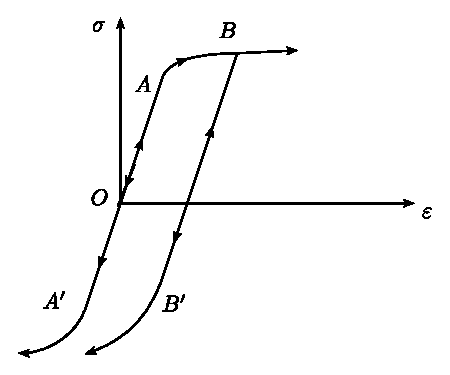
\includegraphics{../images/T1_Ch10-01.eps}
    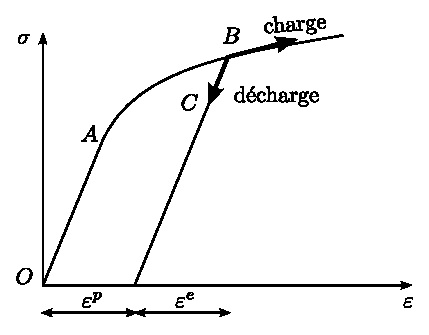
\includegraphics{../images/T1_Ch10-02.eps}
\end{center}

Au départ, le matériau se comporte comme un matériau élastique, tant que l'on ne sort pas du domaine élastique initial 
\begin{equation}
    \sigma_{A'} < \sigma < \sigma_A \quad \sigma = E \varepsilon
    \label{eq:Ch10-001}
\end{equation}
avec en général $\sigma_{A'} = - \sigma_A$.
Si l'on charge au delà du seuil, alors apparaissent les déformations plastiques.
Si, arrivé au point $B$, on relâche la contrainte, alors on redescend le long de la droite $BB'$, et le comportement redevient élastique, avec une déformation résiduelle $\varepsilon^p$, et tant que l'on reste dans le nouveau domaine élastique, on a 
\begin{equation}
    \sigma_{B'} < \sigma <\sigma_B \quad \sigma=E \varepsilon^e \quad \varepsilon = \varepsilon^e + \varepsilon^p
    \label{eq:Ch10-002}
\end{equation}
avec en général $\sigma_{B'}\neq - \sigma_{B}$, et même $|\sigma_{B'}|<|\sigma_{A'}|$ (effet Bauschinger). 

Ainsi, on peut à chaque instant décomposer la déformation $\varepsilon$ en une partie élastique $\varepsilon^e$ et une partie plastique ou résiduelle $\varepsilon^p$.
Dans le domaine élastique, la déformation plastique reste constante 
\begin{equation}
    \sigma_{B'} < \sigma <\sigma_B \quad \ud \varepsilon^p = 0
    \label{eq:Ch10-003}
\end{equation}
tandis que si l'on est sur le seuil, $\sigma = \sigma_B$ par exemple, alors on peut avoir un processus de charge avec déformation plastique ou un processus de décharge (retour dans la zone élastique) sans déformation plastique 
\begin{equation}
    \sigma = \sigma_B 
    \begin{cases}
        \ud \alpha \geq 0, \quad \ud \varepsilon^p \geq 0, \quad \ud \sigma_B = K \ud \varepsilon^p \\
        \ud \alpha < 0, \quad \ud \varepsilon^p = 0, \quad \ud \sigma_B = 0
    \end{cases}
    \label{eq:Ch10-004}
\end{equation}
la constante $K$ étant un «~module d'écrouissage~».

On peut simplifier ce comportement élasto-plastique avec écrouissage par un 	comportement idéalisé.
Le modèle le plus simple est celui de la plasticité parfaite, c'est-à-dire sans écrouissage.
Le domaine élastique reste alors fixe
\begin{center}
    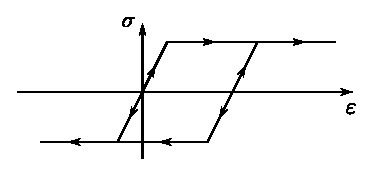
\includegraphics{../images/T1_Ch10-03.eps}
    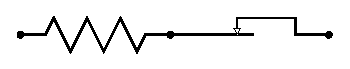
\includegraphics{../images/T1_Ch10-04.eps}
\end{center}
C'est le modèle rhéologique décrit au paragraphe~\ref{ssec:Ch04-2.2}.
D'après~\eqref{eq:Ch04-039} et \eqref{eq:Ch04-040}, la loi de comportement de ce modèle peut s'écrire sous la forme 
\begin{equation}
    \sigma = E \varepsilon^e \quad, \quad |\sigma| \leq \sigma_o \quad, \quad \varepsilon = \varepsilon^o + \varepsilon^p 
    \label{eq:Ch10-005}
\end{equation}
\begin{equation}
    \left\{
    \begin{aligned}
        &\dot{\varepsilon}^p = 0  \text{ si } |\sigma| < \sigma_0 \text{ ou } |\sigma| = \sigma_0, \ |\sigma|' < 0 \\
        &\left.
        \begin{aligned}
            \dot{\varepsilon}^p \geq 0 & \text{ si } \sigma = \sigma_0, \dot{\sigma} = 0 \\
            \dot{\varepsilon}^p \leq 0 & \text{ si } \sigma = - \sigma_0, \dot{\sigma} = 0
        \end{aligned}
        \right\} \text{ charge}
    \end{aligned}
    \right.
    \label{eq:Ch10-006}
\end{equation}
Par analogie avec ce que nous avons fait au paragraphe~\ref{ssec:Ch04-1.2} pour les lois de frottement \eqref{eq:Ch04-014} ou pour les conditions de contact unilatéral \eqref{eq:Ch04-013}, nous pouvons réécrire \eqref{eq:Ch10-006} sous une forme plus synthétique 
\begin{equation}
    \dot{\varepsilon}^p = \lambda \text{sign} (\sigma)
    \label{eq:Ch10-007}
\end{equation}
\begin{equation}
    \left\{
    \begin{aligned}
        \text{si } |\sigma| < \sigma_0, & \lambda = 0 \\
        \text{si } |\sigma| = \sigma_0, & \lambda \geq 0, \ |\sigma|' \leq 0, \ \lambda \dot{\sigma} = 0
    \end{aligned}
    \right.
    \label{eq:Ch10-008}
\end{equation}

On utilise aussi parfois, notamment pour des problèmes qui supposent de grandes déformations plastiques (mise en forme des métaux), l'approximation rigide--plastique, qui revient à négliger les déformations élastiques. 
\begin{multicols}{2}
    \begin{center}
        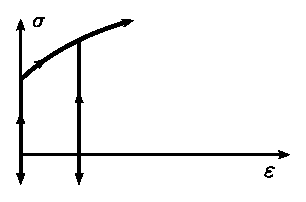
\includegraphics{../images/T1_Ch10-05}

        avec écrouissage
    \end{center}
    \begin{center}
        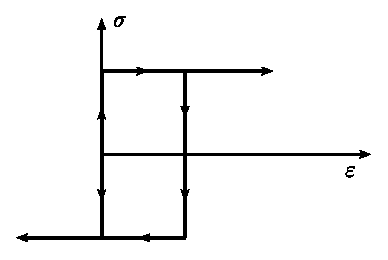
\includegraphics{../images/T1_Ch10-06}

        parfaitement plastique
    \end{center}
\end{multicols}

\subsection{Plasticité parfaite}
Nous nous limiterons désormais à la plasticité parfaite, qui conduit à la théorie classique de la plasticité.
Cette théorie peut en effet être poussée assez loin, et permet d'obtenir de nombreux résultats. 

La définition du seuil de plasticité dans une théorie tridimensionnelle a fait l'objet du paragraphe~\ref{sec:Ch05-3}.
De manière générale, le domaine élastique est défini par 
\begin{equation}
    f\left( \sigma_{ij} \right) \leq 0
    \label{eq:Ch10-009}
\end{equation}
où $f$ est la fonction seuil ou fonction de fluage.
En plasticité parfaite, le domaine élastique ne change pas, et cette fonction est définie une fois pour toutes.
Dans le cas isotrope, on a discuté au paragraphe~\ref{ssec:Ch05-3.1} la forme que prenait ce critère pour les métaux 
\begin{equation}
    f\left( s_{ij} \right) = f\left( J_2,J_3 \right) \leq 0
    \label{eq:Ch10-010}
\end{equation}
et les deux critères les plus utilisés sont le critère de von Mises 
\begin{equation}
    \frac{1}{2} s_{ij} s_{ij} \leq \frac{\sigma_e^2}{3}
    \label{eq:Ch10-011}
\end{equation}
et le critère de Tresca (paragraphe~\ref{ssec:Ch05-3.1}) 
\begin{equation}
    \left( \sigma_1 - \sigma_3 \right) \leq \sigma_e \quad \left( \sigma_1 \geq \sigma_2 \geq \sigma_3 \right)
    \label{eq:Ch10-012}
\end{equation}

Pour les sols, la pression hydrostatique intervient essentiellement dans le critère, et on obtient en général de bons résultats en prenant le critère de Coulomb 
\begin{defn}[Critère de Coulomb]
    \begin{equation}
        |\vec{T}_t| < c - T_n \tan \varphi
        \label{eq:Ch10-013}
    \end{equation}
\end{defn}
où $c$ est «~la cohésion~» et $\varphi$ «~l'angle de frottement interne~».
En particulier, pour un sol sans cohésion,$ c = 0$ (cas des matériaux granulaires comme le sable), le critère de Coulomb exprime simplement une loi de frottement coulombien sur chaque facette. 
\begin{multicols}{2}
    \centering
    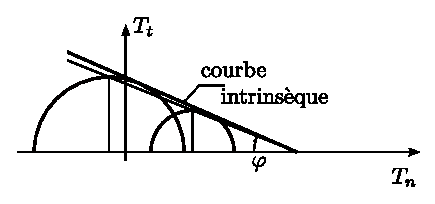
\includegraphics{../images/T1_Ch10-07}
    \columnbreak
    C'est un critère du type~\eqref{eq:Ch05-062}, la courbe intrinsèque étant une droite. 
\end{multicols}

Comme dans le cas unidimensionnel, nous décomposons la déformation 
en une partie élastique et une partie plastique 
\begin{equation}
    \varepsilon_{ij} = \varepsilon_{ij}^e + \varepsilon_{ij}^p
    \label{eq:Ch10-014}
\end{equation}
et la contrainte est donnée par une loi élastique en fonction des déformations élastiques 
\begin{equation}
    \sigma_{ij} = A_{ijkh} \varepsilon_{kh}^e
    \label{eq:Ch10-015}
\end{equation}
et il reste à compléter la théorie par une loi d'écoulement plastique donnant l'évolution de la déformation plastique au cours du temps.
Il convient donc de généraliser la loi \eqref{eq:Ch10-007}, \eqref{eq:Ch10-008} du cas unidimensionnel.
Auparavant, reprenons, dans le cas de l'élasto-plasticité, le bilan thermodynamique exprimé par \eqref{eq:Ch01-060}.
Compte-tenu de \eqref{eq:Ch10-014} et \eqref{eq:Ch10-015}, nous pouvons écrire 
\begin{equation}
    \begin{aligned}
        & \sigma_{ij} D_{ij} = \sigma_{ij} \dot{\varepsilon}_{ij} = \sigma_{ij} \dot{\varepsilon}_{ij}^e + \sigma_{ij} \dot{\varepsilon}_{ij}^p \\
        & \sigma_{ij} \dot{\varepsilon}_{ij}^e = A_{ijkh} \varepsilon_{kh}^e \dot{\varepsilon}_{ij}^e = \frac{\ud w}{\ud t}
    \end{aligned}
    \label{eq:Ch10-016}
\end{equation}
où $w$ est l'énergie de déformation élastique
\begin{equation}
    w = \frac{1}{2} A_{ijkh} \varepsilon_{ij}^e \varepsilon_{kh}^e
    \label{eq:Ch10-017}
\end{equation}
ce qui permet d'identifier \eqref{eq:Ch10-016} à \eqref{eq:Ch01-059} avec 
\begin{equation}
    \rho u = w \quad,\quad \varphi = \sigma_{ij} \dot{\varepsilon}_{ij}^p
    \label{eq:Ch10-018}
\end{equation}
La puissance «~élastique~» se transforme en énergie interne élastique, tandis que la puissance «~plastique~» est dissipée.
Le second principe de la thermodynamique donne alors l'inégalité 
\begin{equation}
    \sigma_{ij} \dot{\varepsilon}_{ij}^p \geq 0
    \label{eq:Ch10-018}
\end{equation}
restriction thermodynamique sur la loi d'écoulement plastique. 

\subsection{Potentiel plastique} \label{ssec:Ch10-1.3}
\begin{center}
    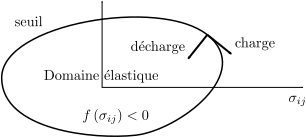
\includegraphics{../images/T1_Ch10-08}
\end{center}
Comme dans le cas unidimensionnel, la déformation plastique reste constante si l'on est en évolution élastique, c'est-à-dire si l'on est dans le domaine élastique($f<0$) ou sur le seuil $f=O$ si l'on a un processus de décharge ($\dot{f} < 0$) 
\begin{equation}
    \dot{\varepsilon}_{ij}^p = 0
    \begin{cases}
        \text{si } f < 0 & \text{ domaine élastique} \\
        \text{si } f = 0, & \dot{f}<0 \text{ décharge}
    \end{cases}
    \label{eq:Ch10-019}
\end{equation}
La déformation plastique ne varie donc que sur le seuil et dans un processus de charge ($f=0$, $\dot{f}=0$).
La loi d'évolution est alors habituellement définie par 
\begin{Principe}[Principe du travail maximal]
    Dans un état de contraintes $\sigma_{ij}$, le taux de 
déformation plastique vérifie l'inégalité 
    \begin{equation}
        \left( \sigma_{ij} - {\mathop{\sigma}^{\ast}}_{ij} \right) \dot{\varepsilon}_{ij}^p \geq 0
        \label{eq:Ch10-020}
    \end{equation}
    pour tout $\displaystyle {\mathop{\sigma}^{\ast}}_{ij}$ acceptable, $\displaystyle f\left( {\mathop{\sigma}^{\ast}}_{ij} \right) \leq 0$.
\end{Principe}

En particulier, il s'ensuit que la restriction thermodynamique \eqref{eq:Ch10-018} est automatiquement vérifiée (il suffit de prendre $\displaystyle {\mathop{\sigma}^{\ast}}_{ij}=0$ dans \eqref{eq:Ch10-020}). 

Géométriquement,en se plaçant dans l'espace vectoriel des contraintes (de dimension 6), l'inégalité \eqref{eq:Ch10-020} se traduit par l'inégalité 
\begin{equation}
    \vec{\Sigma^{\ast} \Sigma} \cdot \vec{\ud \varepsilon^p} \geq 0
    \label{eq:Ch10-021}
\end{equation}
où $\Sigma$ est le point représentatif de l'état de contraintes, $\Sigma^{\ast}$ un point quelconque du domaine élastique, et $\vec{\ud \varepsilon^p}$ le vecteur représentatif de l'incrément de déformation plastique. 

Si l'on se place en un point du seuil où le plan tangent est continu, alors, en faisant varier $\Sigma^{\ast}$, on constate que l'inégalité \eqref{eq:Ch10-021} sera vérifiée pour tout $\Sigma^{\ast}$ si-et-seulement-si le vecteur incrément de déformation plastique est 
\begin{center}
    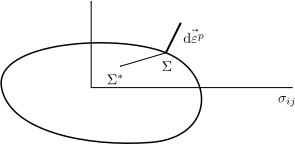
\includegraphics{../images/T1_Ch10-09}
\end{center}
dirigé selon la normale extérieure à la surface seuil en $\Sigma$ 
\begin{equation}
    \dot{\varepsilon}_{ij}^p = \lambda \frac{\partial f}{\partial \sigma_{ij}} \quad,\quad \lambda \geq 0
    \label{eq:Ch10-022}
\end{equation}
La fonction seuil est un «~potentiel plastique~».
On tire également de \eqref{eq:Ch10-020} la propriété de convexité du domaine élastique 
\begin{multicols}{2}
    \begin{center}
        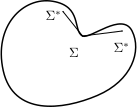
\includegraphics{../images/T1_Ch10-10}
    \end{center}
    \columnbreak
    En effet, si ce domaine n'est pas convexe, alors on constate aisément qu'il est impossible de trouver un vecteur $\vec{\ud \varepsilon^p}$ vérifiant \eqref{eq:Ch10-021} pour tout $\Sigma^{\ast}$.
\end{multicols}
Ainsi, on tire du principe du travail maximal les propriétés de convexité (du domaine élastique) et de normalité (de $\vec{\ud \varepsilon^p}$ à la frontière seuil). 

Par analogie avec ce que nous avons fait au paragraphe~\ref{ssec:Ch04-1.2} pour la condition de frottement, nous pouvons réécrire la loi d'écoulement plastique sous la forme 
\begin{equation}
    \left\{
    \begin{aligned}
        \dot{\varepsilon}_{ij}^p = 0 & \text{si} & f\left( \sigma_{ij} \right) < 0 \\
        \dot{\varepsilon}_{ij}^p = \lambda \frac{\partial f}{\partial \sigma_{ij}} & \text{si} & f\left( \sigma_{ij} \right) = 0
    \end{aligned}
    \right.
    \label{eq:Ch10-023}
\end{equation}
\[
\lambda \geq 0 \quad,\quad \dot{f} \leq 0 \quad,\quad \lambda \dot{f} = 0
\]
et la distinction entre processus de charge et de décharge s'effectue automatiquement par le jeu des deux inégalités et de l'inégalité sur $\lambda$ et $\dot{f}$.
Cela peut sembler bien compliqué, c'est néanmoins la «~bonne formulation mathématique~» qui permet de démontrer de nombreux résultats. 

En particulier, si le critère ne dépend pas de la pression hydrostatique forme \eqref{eq:Ch10-010} alors il résulte de \eqref{eq:Ch10-023} que 
\begin{equation}
    \dot{\varepsilon}_{ii}^p = 0
    \label{eq:Ch10-024}
\end{equation}
Les déformations plastiques se font à volume constant (incompressibilité plastique). 

Si la surface seuil présente un point anguleux le cas du critère de Tresca -- alors le principe du travail maximal montre que le vecteur $\vec{\ud \varepsilon^p}$ est dans le cône des normales  
\begin{center}
    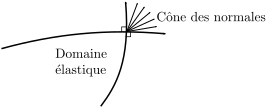
\includegraphics{../images/T1_Ch10-11}
\end{center}

Le principe du travail maximal est une hypothèse qui sera ou non vérifiée selon les matériaux.
Elle est vérifiée en première approximation pour les métaux; elle n'est pas vérifiée par contre pour les sols.
Ce principe permet d'engendrer une classe de modèles: les matériaux standard, qui permettent de traiter de nombreux problèmes.
Les conclusions obtenues à partir de ce type de modèle seront plus ou moins valables selon les problèmes.

Dans le cas du critère de von Mises \eqref{eq:Ch10-011}, on obtient 
\begin{equation}
    \dot{\varepsilon}_{ij}^p = \lambda s_{ij}
    \label{eq:Ch10-025}
\end{equation}
et, par combinaison avec \eqref{eq:Ch10-015}, on a 
\begin{equation}
    \dot{\varepsilon}_{ij} = \Lambda_{ijkh} \dot{\sigma}_{kh} + \lambda s_{ij}
    \label{eq:Ch10-026}
\end{equation}
loi de comportement incrémentale de la plasticité. 

\section{Exemples de problèmes} \label{sec:Ch10-2}
\subsection{Flexion d'une poutre} \label{ssec:Ch10-2.1}
Considérons un arbre élastoplastique, et soumettons le à un moment 
de flexion $\mathcal{M}$ croissant (voir paragraphe~\ref{ssec:Ch07-1.1}, problèmes 5 et 6).
Au départ, la solution élastique du paragraphe~\ref{ssec:Ch07-1.3} est valable, et elle le reste tant que 
\begin{equation}
    \mathcal{M} < \mathcal{M}_e = \frac{\sigma_e J}{\eta}
    \label{eq:Ch10-027}
\end{equation}
Au delà de $\mathcal{M}_e$, une zone plastique se développe à l'extérieur de la poutre, tandis qu'au milieu subsiste une âme élastique.
En supposant que, en chaque point, l'état de contraintes reste un état de traction simple \eqref{eq:Ch07-013}, nous sommes amenés à prendre 
\begin{equation}
    \sigma_{11} = 
    \begin{cases}
        \displaystyle -\sigma_e & \displaystyle \xi \leq x_2 \leq  \frac{h}{2} \\
        \displaystyle -\frac{\sigma_e x_2}{\xi} & \displaystyle -\xi \leq x_2 \leq \xi \\
        \displaystyle +\sigma_e & \displaystyle -\frac{h}{2} \leq x_2 \leq -\xi
    \end{cases}
    \label{eq:Ch10-028}
\end{equation}
en supposant la poutre symétrique par rapport à l'axe $x_3$.

\begin{multicols}{2}
    Ce champ de contraintes vérifie les équations d'équilibre et les CL sur la surface latérale.
    Il vérifie aussi si les CL sur les extrémités avec
    \[
    \mathcal{M} = - \iint_{\Sigma} x_2 \sigma_{11} \ud x_2 \ud x_3
    \]
    \columnbreak
    \begin{center}
        \includegraphics{../images/T1_Ch10-12}
    \end{center}
\end{multicols}
et si on introduit la fonction $b\left( x_2 \right)$ donnant la largeur de la poutre en fonction de $x_2$
\begin{equation}
    \mathcal{M} = 2 \sigma_e \left\{ \int_0^{\xi} \frac{b(x_2)x_2^2}{\xi} \ud x_2 + \int_{\xi}^{h/2} b(x_2)x_2 \ud x_2 \right\} = \mathcal{M} \left( \xi \right)
    \label{eq:Ch10-029}
\end{equation}
où la fonction $\mathcal{M}(\xi)$ est une fonction qui croît de $\mathcal{M}_e$ donné par \eqref{eq:Ch10-027} à $\mathcal{M}_l$ donné par 
\begin{equation}
    \mathcal{M}_l = 2 \sigma_e \int_0^{h/2} b(x_2) x_2 \ud x_2
    \label{eq:Ch10-030}
\end{equation}
lorsque $\xi$ décroît de $h/2$ à $0$, c'est-à-dire lorsque la zone plastique s'étend jusqu'à occuper tout $\Sigma$.

Il reste à calculer les déplacements.
Dans la zone élastique, le calcul du paragraphe~\ref{ssec:Ch07-1.3} reste valable en remplaçant $\mathcal{M}/J$ par $\sigma_e/\xi$, et la relation~\eqref{eq:Ch07-034} devient 
\begin{equation}
    \kappa = \frac{\sigma_e}{E \xi}
    \label{eq:Ch10-031}
\end{equation}
qui, combiné avec \eqref{eq:Ch10-029}, donne la relation entre le moment et la courbure. 

\begin{center}
    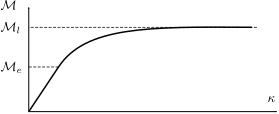
\includegraphics{../images/T1_Ch10-13}
\end{center}
\begin{center}
    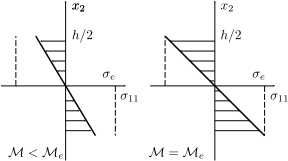
\includegraphics{../images/T1_Ch10-14a}

    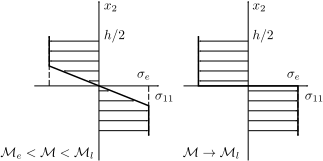
\includegraphics{../images/T1_Ch10-14b}
\end{center}
Il reste à étendre cette solution au domaine plastique, par intégration de \eqref{eq:Ch10-023}.
Cela pose davantage de problèmes, mais il est possible de calculer un champ de déplacements répondant au problème.
Ce champ n'est cependant pas unique: en général, on n'a pas unicité du champ de déplacements en plasticité. 

Finalement, le comportement é1astop1astique d'une poutre en flexion est le suivant 
\begin{itemize}
    \item comportement élastique pour $\mathcal{M}<\mathcal{M}_e$
    \item au delà de $\mathcal{M}_e$: apparition d'une zone plastique, mais les déformations plastiques restent limitées ou «~contenues~» par le noyau élastique. 
    \item pour $\mathcal{M} \rightarrow \mathcal{M}_l$, le noyau élastique disparaît, et les déformations plastiques n'étant plus limitées, il y a ruine de la structure. 
\end{itemize}

\subsection{Réservoir sphérique} \label{ssec:Ch10-2.2}
Reprenons en élastoplasticité le problème du réservoir sphérique que nous avons résolu, en élasticité, au paragraphe~\ref{ssec:Ch06-2.2}.
Si l'on augmente progressivement la pression intérieure $p$, alors la solution élastique reste valable jusqu'à la pression 
\begin{equation}
    p = p_e = \frac{2\sigma_e}{3} \left( 1 - \frac{a^3}{b^3} \right)
    \label{eq:Ch10-032}
\end{equation}
Au delà, une zone plastique apparaît à l'inrérieur du réservoir. 
\begin{multicols}{2}
    \begin{center}
        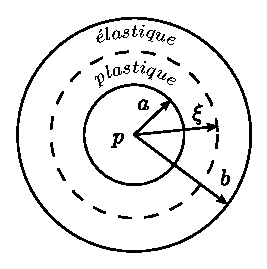
\includegraphics{../images/T1_Ch10-15}
    \end{center}
    \columnbreak
    Par raison de symétrie, cette zone sera limitée par une sphère $r=\xi$.
\end{multicols}
Dans la zone élastique, $\xi \leq r \leq b$, l'analyse du paragraphe~\ref{ssec:Ch06-2.2} subsiste, et le tenseur des contraintes est donné par 
\begin{equation}
    \sigma_{ij} = \left( 3 K \alpha + \frac{2\mu \beta}{r^3} \right) \delta_{ij} - \frac{6\mu \beta}{r^3} \frac{x_ix_j}{r^2}
    \label{eq:Ch10-033}
\end{equation}
$\alpha$ et $\beta$ étant deux constantes à déterminer.

Dans la zone plastique, $a<r<\xi$, d'après la symétrie sphérique du problème, le tenseur des contraintes aura la forme suivante 
\begin{equation}
    \sigma_{ij} = \left[ \pi(r) + \tau(r) \right] \delta_{ij} - 3 \tau(r) \frac{x_ix_j}{r^2}
    \label{eq:Ch10-034}
\end{equation}
où $\pi(r)$ représente la partie sphérique du tenseur des contraintes, et $\tau(r)$ son déviateur.
Ce tenseur est de révolution autour de la direction radiale, et les contraintes principales sont 
\begin{equation}
    \sigma_1 = \sigma_2 = \pi(r) + \tau(r) \quad,\quad \sigma_3 = \pi - 2\tau(r)
    \label{eq:Ch10-035}
\end{equation}
Les équations d'équilibre appliquées à \eqref{eq:Ch10-034} donnent 
\begin{equation}
    2\tau'(r) + \frac{6\tau(r)}{r} - \pi'(r) = 0
    \label{eq:Ch10-036}
\end{equation}
équation différentielle reliant les deux fonctions $\pi(r)$ et $\tau(r)$. 
D'autre part, dans la zone plastique on doit avoir 
\[
\frac{1}{2} s_{ij} s_{ij} = 3 \tau^2 = \frac{\sigma_e^2}{3}
\]
en adoptant par exemple le critère de von Mises (comme on l'a vu en \ref{ssec:Ch06-2.2} le critère de Tresca donnerait-le même résultat).
On en tire donc 
\begin{equation}
    \tau = + \frac{\sigma_e}{3}
    \label{eq:Ch10-037}
\end{equation}
(le choix du signe se fait par continuité avec la solution élastique du paragraphe~\ref{ssec:Ch06-2.2}).
En reportant dans \eqref{eq:Ch10-036} et en intégrant, on obtient 
\begin{equation}
    \pi = 2 \sigma_e \log r + \text{Cte}
    \label{eq:Ch10-038}
\end{equation}
Ainsi, dans le domaine plastique 
\begin{equation}
    \sigma_{ij} = 2 \sigma_e \left( \log r + \gamma \right) \delta_{ij} - \sigma_e \frac{x_ix_j}{r^2}
    \label{eq:Ch10-039}
\end{equation}
\begin{equation}
    \sigma_1 = \sigma_2 = 2 \sigma_e \left( \log r + \gamma \right), \quad \sigma_3 = 2 \sigma_e \left( \log r + \gamma - \frac{1}{2} \right)
    \label{eq:Ch10-040}
\end{equation}
où $\gamma$ est une constante d'intégration.
Ainsi, le champ de contraintes, défini par \eqref{eq:Ch10-033} pour $\xi \leq r \leq b$ et par \eqref{eq:Ch10-039} pour $a \leq \xi \leq r$, dépend de trois constantes d'intégration $\alpha$, $\beta$, $\gamma$.
Ces trois constantes d'intégration s'obtiennent en écrivant la CL en $r=b$ et la condition de continuité de $\sigma_1$, $\sigma_2$ et $\sigma_3$ au travers de la surface $r=\xi$.
Remarquons ici que la condition de discontinuité \eqref{eq:Ch01-022} impose seulement la continuité de $\sigma_3$; cependant, en plasticité, on doit écrire qu'à la frontière élasto-plastique, l'état élastique est un état limite, ce qui revient à écrire la continuité de $\sigma_1$ et $\sigma_2$.
Les trois constantes d'intégration étant ainsi déterminées, la CL en $r = a$ donne la valeur de $p$ qui correspond à $\xi$, d'où la fonction $p(\xi)$ qui croît de $p_e$ à $p_l$ lorsque $\xi$ croît de $a$ jusqu'à $b$.
La valeur limite $p_l$ de $p$ s'obtient lorsque $\xi=b$, c'est-à-dire lorsque la zone élastique disparaît.
Le champ de contraintes est alors donné par \eqref{eq:Ch10-039}, \eqref{eq:Ch10-040} pour tout $r$.
La CL en $r=b$ donne alors $\gamma$ et il vient 
\begin{equation}
    \sigma_3 = 2 \sigma_e \log \frac{r}{b}
    \label{eq:Ch10-041}
\end{equation}
et en faisant $r=a$ on trouve 
\begin{equation}
    p_l = 2 \sigma_e \log \frac{b}{a}
    \label{eq:Ch10-042}
\end{equation}

Comme en flexion, le réservoir se comporte élastiquement jusqu'à $p_e$.
Au delà de $p_e$ des déformations plastiques apparaissent, mais ces déformations restent contenues par la zone élastique jusqu'à ce que $p$ atteigne la valeur 1imite $p_l$ qui correspond à la ruine du réservoir. 

\section{Méthodes variationnelles} \label{sec:Ch10-3}
\subsection{Le problème en vitesses} \label{ssec:Ch10-3.1}
En plasticité, il n'y a pas relation biunivoque entre les contraintes et les déformations; il est donc tout à fait clair qu'un problème statique régulier, tel que nous l'avons formulé au paragraphe~\ref{ssec:Ch06-1.1}, est automatiquement mal posé. 
En effet, l'état de contraintes et de déformations dans un matériau élasto-plastique ne dépend pas seulement de la sollicitation appliquée à l'instant considéré, mais aussi de tout ce qui s'est passé auparavant.
Par contre, connaissant l'état actuel de contraintes et de déformations, et connaissant la variation de sollicitation, on peut espérer trouver la solution.
Dans le cadre de l'hypothèse quasi-statique, on est donc amené à se poser un problème incrémental (ou problème en vitesses). 

\begin{defn}[Problème incrémental]
    Connaissaht à l'instant $t$ le champ des contraintes $\sigma_{ij}(x,t)$ et le champ des déplacements $u_i(x,t)$, trouver leurs variations vérifiant 
    \begin{itemize}
        \item les équation d'équilibre incrémentales 
            \begin{equation}
                \dot{\sigma}_{ij,j} + \dot{f}_i = 0
                \label{eq:Ch10-043}
            \end{equation}
        \item les conditions aux limites 
            \begin{equation}
                \dot{\sigma}_{ij} n_j|_{S_f} = \dot{T}_i^d
                \label{eq:Ch10-044}
            \end{equation}
            \begin{equation}
                \dot{u}_i|_{S_u} = \dot{u}_i^d
                \label{eq:Ch10-045}
            \end{equation}
        \item la loi de comportement incrémentale 
            \begin{equation}
                \dot{\varepsilon}_{ij} = \Lambda_{ijkh} \dot{\sigma}_{kh} + \dot{\varepsilon}_{ij}^p
                \label{eq:Ch10-046}
            \end{equation}
            avec $\dot{\varepsilon}_{ij}^p$ donné par la loi d'écoulement plastique.
    \end{itemize}
\end{defn}
Si nous acceptons le principe du travail maximal, c'est encore 
un problème bien posé.
\begin{thmn}[Théorème de l'unicité]
    En acceptant le principe du travail maximal, le problème posé plus haut admet une solution unique en $\dot{\sigma}_{ij}$.
\end{thmn}
\begin{proof}
    Supposons en effet qu'il existe deux solutions $\left( \dot{\sigma}_{ij}^1, \dot{u}_i^1 \right)$ et $\left( \dot{\sigma}_{ij}^2, \dot{u}_i^2 \right)$.
    Leur différence
    \begin{equation}
        \dot{\sigma}_{ij}^0 = \dot{\sigma}_{ij}^1 -  \dot{\sigma}_{ij}^2, \quad \dot{u}_i^0 = \dot{u}_i^2 - \dot{u}_i^1
        \label{eq:Ch10-047}
    \end{equation}
    vérifie les équations 
    \begin{equation}
        \dot{\sigma}_{ij,j}^0 = 0, \quad \dot{\sigma}_{ij}^0 n_j|_{S_f} = 0, \quad \dot{u}_i^0 |_{S_u} = 0
        \label{eq:Ch10-048}
    \end{equation}
    (Par contre, elle ne vérifie pas nécessairement la loi de comportement \eqref{eq:Ch10-046} qui est non linéaire).
    En appliquant à $\dot{\sigma}_{ij}^0$ et $\dot{u}_i^0$ le lemme fondamental du paragraphe~\ref{ssec:Ch09-1.1}, on obtient alors 
    \begin{equation}
        \iiint_{\Omega} \dot{\sigma}_{ij}^0 \dot{\varepsilon}_{ij}^0 \ud v = \iiint_{\Omega} \left( \dot{\sigma}_{ij}^2 - \dot{\sigma}_{ij}^1 \right)\left( \dot{\varepsilon}_{ij}^2 - \dot{\varepsilon}_{ij}^1 \right) \ud v = 0
        \label{eq:Ch10-049}
    \end{equation}
    Mais
    \[
    \begin{aligned}
        \left( \dot{\sigma}_{ij}^2 - \dot{\sigma}_{ij}^1 \right)\left( \dot{\varepsilon}_{ij}^2 - \dot{\varepsilon}_{ij}^1 \right) & = \left( \dot{\sigma}_{ij}^2 - \dot{\sigma}_{ij}^1 \right) \left( \dot{\varepsilon}_{ij}^{e,2} - \dot{\varepsilon}_{ij}^{e,1} \right) + \left( \dot{\sigma}_{ij}^2 - \dot{\sigma}_{ij}^1 \right)\left( \dot{\varepsilon}_{ij}^{p,2} - \dot{\varepsilon}_{ij}^{p,1} \right) \\
        & = \Lambda_{ijkh} \left( \dot{\sigma}_{ij}^2 - \dot{\sigma}_{ij}^1 \right) \left( \dot{\sigma}_{kh}^2 - \dot{\sigma}_{kh}^1 \right) + \dot{\sigma}_{ij}^2 \dot{\varepsilon}_{ij}^{p,2} + \dot{\sigma}_{ij}^1 \dot{\varepsilon}_{ij}^{p,1} - \dot{\sigma}_{ij}^2 \dot{\varepsilon}_{ij}^{p,1} - \dot{\sigma}_{ij}^1 \dot{\varepsilon}_{ij}^{p,2}
    \end{aligned}
    \]
    En tout point $x$, on connait le tenseur des contraintes, on connait donc la zone élastique $\Omega_e$ où $f\left( \sigma_{ij} \right) < 0$ et la zone plastique $\Omega_p$ où $f\left( \sigma_{ij} \right) < 0$. 
    Dans la zone élastique, les taux de déformations plastiques sont identiquement nuls.
    Dans la zone plastique, on vérifie directement que, d'après le principe du travail maximal: 
    \begin{flushright}
        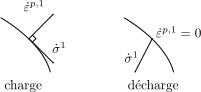
\includegraphics{../images/T1_Ch10-16}
    \end{flushright}
    \begin{equation}
        \dot{\varepsilon}_{ij}^{p,1} \dot{\sigma}_{ij}^1 = 0 \quad \dot{\varepsilon}_{ij}^{p,1} \dot{\sigma}_{ij}^2 \leq 0
        \label{eq:Ch10-050}
    \end{equation}
    Ainsi, on peut écrire à partir de \eqref{eq:Ch10-049}, \eqref{eq:Ch10-050}
    \begin{equation}
        \iiint_{\Omega} \Lambda_{ijkh} \left( \dot{\sigma}_{ij}^2 - \dot{\sigma}_{ij}^1 \right) \left( \dot{\sigma}_{kh}^2 - \dot{\sigma}_{kh}^1 \right) \ud v = \iiint_{\Omega_p} \left( \dot{\sigma}_{ij}^2 \dot{\varepsilon}_{ij}^{p,1} + \dot{\sigma}_{ij}^1 \dot{\varepsilon}_{ij}^{p,2} \right) \ud v \leq 0
        \label{eq:Ch10-051}
    \end{equation}
    or, $\Lambda_{ijkh}$ est défini positif.
    On obtient donc
    \begin{equation}
        \iiint_{\Omega} \Lambda_{ijkh} \left( \dot{\sigma}_{ij}^2 - \dot{\sigma}_{ij}^1 \right) \left( \dot{\sigma}_{kh}^2 - \dot{\sigma}_{kh}^1 \right) \ud v = 0
        \label{eq:Ch10-052}
    \end{equation}
    \begin{equation}
        \dot{\sigma}_{ij}^2 = \dot{\sigma}_{ij}^1
        \label{eq:Ch10-053}
    \end{equation}
\end{proof}

Par contre, on ne sait pas démontrer l'unicité des déformations. 
Ces problèmes sont des problèmes mathématiques difficiles et encore mal connus.

On sait également démontrer des théorèmes variationnels analogues à ceux des paragraphes~\ref{ssec:Ch09-1.2} et \ref{ssec:Ch10-1.3}, qui donnent naissance à des méthodes numériques de solution du problème incrémental.
La résolution d'un problème élasto-plastique quasi-statique se fait donc pas à pas, par résolution d'une suite de problèmes en vitesses.
Mais il est important de remarquer que pour toutes ces questions, la formulation de la loi d'écoulement plastique par le principe du travail maximal joue un rôle essentiel. 

\subsection{Introduction a l'analyse limite} \label{ssec:Ch10-3.2}
Nous considérons un problème où le chargement dépend d'un seul paramètre 
\begin{equation}
    \left\{
    \begin{aligned}
        S_u = \emptyset \text{ ou } u_i^d = 0 \\
        T_i^d = \lambda T_i^{d0}, \quad f_i = \lambda f_i^0
    \end{aligned}
    \right.
    \label{eq:Ch10-054}
\end{equation}
Pour les problèmes envisagés au paragraphe~\ref{sec:Ch10-2}, on  a $\lambda = \mathcal{M}$ pour la poutre en flexion et $\lambda=p$ pour le réservoir sphérique.  

Si l'on fait croître le chargement, on obtient toujours le même comportement.
Jusqu'à $\lambda=\lambda_e$ la solution élastique convient.
Au delà apparaît une zone plastique qui progresse au fur et à mesure que $\lambda$ augmente, et jusqu'à ce que pour $\lambda-\lambda_l$ on ait ruine de la structure par déformations plastiques illimitées. 

La charge correspondant à $\lambda=\lambda_l$ est appelée «~charge limite~».
C'est la charge maximale supportable et, d'un point de vue pratique, c'est le résultat le plus intéressant et le plus significatif d'un calcul en plasticité.
On a donc cherché à développer des méthodes permettant de calculer directement cette charge limite, sans résolution complète du problème élasto-plastique: c'est le domaine de l'analyse limite. 

La théorie s'appuie sur deux théorèmes fondamentaux. 
\begin{deff}
    Un champ de contraintes $\hat{\sigma}_{ij}$ sera un champ licite pour un chargement $(f_i,T_i^d)$ s'il est statiquement admissible et si en tout point il vérifie le critère de plasticité. 
\end{deff}
\begin{deff}
    Un champ de vitesses $\tilde{\dot{u}}_i$ sera un champ cinématiquement et plastiquement admissible (CCPA) s'il est cinématiquement admissible et si en chaque point il existe un  tenseur de contraintes $\tilde{\sigma}_{ij}$ tel que $\tilde{\dot{\varepsilon}}_{ij}$ puisse être la déformation plastique associée.  
\end{deff}

Dans le cas des métaux par exemple, cette dernière condition revient simplement à imposer la condition 
\begin{equation}
    \tilde{\dot{\varepsilon}}_{ii} = 0
    \label{eq:Ch10-055}
\end{equation}
On définit alors la fonction de dissipation 
\begin{equation}
    D\left( \tilde{\dot{\tens{\varepsilon}}}_p \right) = \tilde{\sigma}_{ij} \tilde{\dot{\varepsilon}}_{ij}^p
    \label{eq:Ch10-056}
\end{equation}
fonction définie sans ambiguïté, bien qu'il puisse exister plusieurs $\tilde{\sigma}_{ij}$ compatibles avec $\tilde{\dot{\varepsilon}}_{ij}^p$.
Pour le critère de von Mises par exemple 
\begin{equation}
    D\left( \tilde{\dot{\tens{\varepsilon}}}_p \right) = \frac{2}{3} \sigma_e \tilde{\varepsilon}_{ij}^p \tilde{\varepsilon}_{ij}^p \quad \left( \dot{\varepsilon}_{ii}^p = 0 \right)
    \label{eq:Ch10-057}
\end{equation}
On peut alors démontrer les deux thêorèmes suivants.
\begin{thmn}[Théorème statique]
    S'il existe un champ de contraintes licite pour le chargement $\left( f_i, T_i^d \right)$, alors la structure peut supporter ce chargement.
\end{thmn}
\begin{thmn}[Théorème cinématique]
    S'il existe un CCPA tel que 
    \begin{equation}
        \iiint_{\Omega} f_i \tilde{\dot{u}}_i \ud v + \iint_{S_f} T_i^d \tilde{\dot{u}}_i \ud S > \iiint_{\Omega} D \left( \tilde{\dot{\varepsilon}}_{ij} \right) \ud v
        \label{eq:Ch10-058}
    \end{equation}
    alors la structure ne peut pas supporter le chargement $\left( f_i, T_i^d \right)$.
\end{thmn}
Le premier théorème permet de construire des bornes inférieures de la charge limite.
En effet, soit $\hat{\sigma}_{ij}^0$ un CSA pour le chargement $\left( f_i, T_i^d \right)$.
Alors, le champ $\lambda \hat{\sigma}_{ij}^0$ sera CSA pour le chargement $\left( f^0_i, T_i^{d0} \right)$.
En choisissant pour $\lambda$ la plus grande valeur conduisant à un champ licite 
\begin{equation}
    \hat{\lambda} = \sup \left\{ \lambda | f\left( \lambda \hat{\sigma}_{ij}^0 \right) \leq 0\ \forall x \right\}
    \label{eq:Ch10-059}
\end{equation}
alors, le théorème statique permet d'affirmer que $\hat{\lambda}$ est une borne inférieure de la charge limite. 

De la même manière, le second théorème permet d'obtenir des bornes supêrieures de la charge limite.
Soit en effet $\tilde{\dot{u}}_i$ un CCPA, alors la structure ne pourra pas supporter les chargements vérifiant \eqref{eq:Ch10-058}.
La quantité 
\begin{equation}
    \tilde{\lambda} = \iiint_{\Omega} D \left( \tilde{\dot{\varepsilon}}_{ij} \right) \ud v \left\{ \iiint_{\Omega} f_i^0 \tilde{\dot{u}}_i \ud v + \iint_{S_f} T_i^{d0} \tilde{\dot{u}}_i \ud S \right\}^{-1}
    \label{eq:Ch10-060}
\end{equation}
est donc une borne supérieure de $\lambda_l$.
On en déduit un encadrement 
\begin{equation}
    \hat{\lambda} \leq \lambda_l \leq \tilde{\lambda}
    \label{eq:Ch10-061}
\end{equation}
qui permet d'approcher relativement simplement la charge limite. 
On notera l'analogie de cette méthode avec celle présentée en élasticité. 

L'analyse limite est utilisée:
\begin{itemize}
    \item en mécanique des structures, car la charge limite caractérise bien la capacité de résistance d'une structure -- bien mieux en tout cas que la charge élastique $\lambda_e$.
        La tendance actuelle de la règlementation en matière de calcul d'ouvrage consiste à substituer un calcul plastique au calcul élastique traditionnel. 
    \item pour les problèmes mise en forme des métaux (laminage, filage, etc.), car elle permet d'évaluer les efforts nécessaires. 
    \item en mécanique des sols, pour calculer la capacité de résistance d'un ouvrage.
        Il convient alors d'agir avec précaution, car les théorèmes que nous avons énoncés supposent le principe du travail maximal, principe non vérifié pour les sols. 
\end{itemize}
